\documentclass[]{article}

% ------
% Fonts and typesetting settings
\usepackage[sc]{mathpazo}
\usepackage[T1]{fontenc}
\linespread{1.05} % Palatino needs more space between lines
\usepackage{microtype}
\usepackage{amsmath}

% ------
% Page layout
\usepackage[hmarginratio=1:1,top=30mm,bottom=30mm,columnsep=20pt]{geometry}
\usepackage[font=it]{caption}
\usepackage{paralist}
%\usepackage{multicol}

\usepackage{graphicx}
\usepackage{color}
\usepackage{tabularx}
\usepackage{multirow}

\usepackage{capt-of}

% \usepackage[ngerman]{babel}

% ------
% Lettrines
\usepackage{lettrine}

% ------
% Abstract
\usepackage{abstract}
	\renewcommand{\abstractnamefont}{\normalfont\bfseries}
	\renewcommand{\abstracttextfont}{\normalfont\small\itshape}


% ------
% Titling (section/subsection)
\usepackage{titlesec}
\renewcommand\thesection{\Roman{section}}
\titleformat{\section}[block]{\large\scshape\centering}{\thesection.}{1em}{}


% ------
% Header/footer
\usepackage{fancyhdr}
	\pagestyle{fancy}
	\fancyhead{}
	\fancyfoot{}
	\fancyhead[C]{Post-quantum cryptography $\bullet$ Winter 2018/19 $\bullet$ RheinMain University of Applied Sciences}
	\fancyfoot[RO,LE]{\thepage}


% ------
% Maketitle metadata
\title{\vspace{-7mm}%
	\fontsize{24pt}{10pt}\selectfont
	\textbf{Re-implementation of the Picnic-signaturescheme in Python}
	}	
\author{%
	\large
	\textsc{Thorsten Knoll} \\[2mm]
	\normalsize	info@thorstenknoll.de \\[2mm]
	\normalsize March, 2019
	%\vspace{-5mm}
	}
\date{}

\usepackage[utf8]{inputenc}

\usepackage{hyperref}

%%%%%%%%%%%%%%%%%%%%%%%%
\begin{document}

\maketitle
\thispagestyle{fancy}

%\begin{abstract}
%\noindent Abstract goes here
%\end{abstract}

\section{Introduction}
\subsection{Post-quantum cryptography, NIST and Picnic}
Quantum computers are experiencing fast development and seem to be available within a timeframe of the next few decades. One of their properties will be to break huge parts of modern cryptography. Especially the discrete logarithm and prime-factorisation loose their trapdoor funcionality in regards to the efficient quantum algorithms from Grover and Shor. Therefore the need for new cryptographic algorithms arises, beeing save in regards to the availability of quantum computers. This field of research goes with the name "Post-quantum cryptography" (PQC). The american National Institute of Standards and Technology (NIST) called out a challenge to find the next PQC standards. This challenge is in round two of three at the time of writing this document. 69 submissions from round one were reduced to 26 candidates in round two of the challenge. These 26 candidates got announced by NIST not long ago at the end of january 2019. One of the submissions surviving the first round is the Picnic signaturescheme.
\subsection{Evaluation and categorization}
\subsection{Learning PQC}
\begin{figure}[htbp]
\center
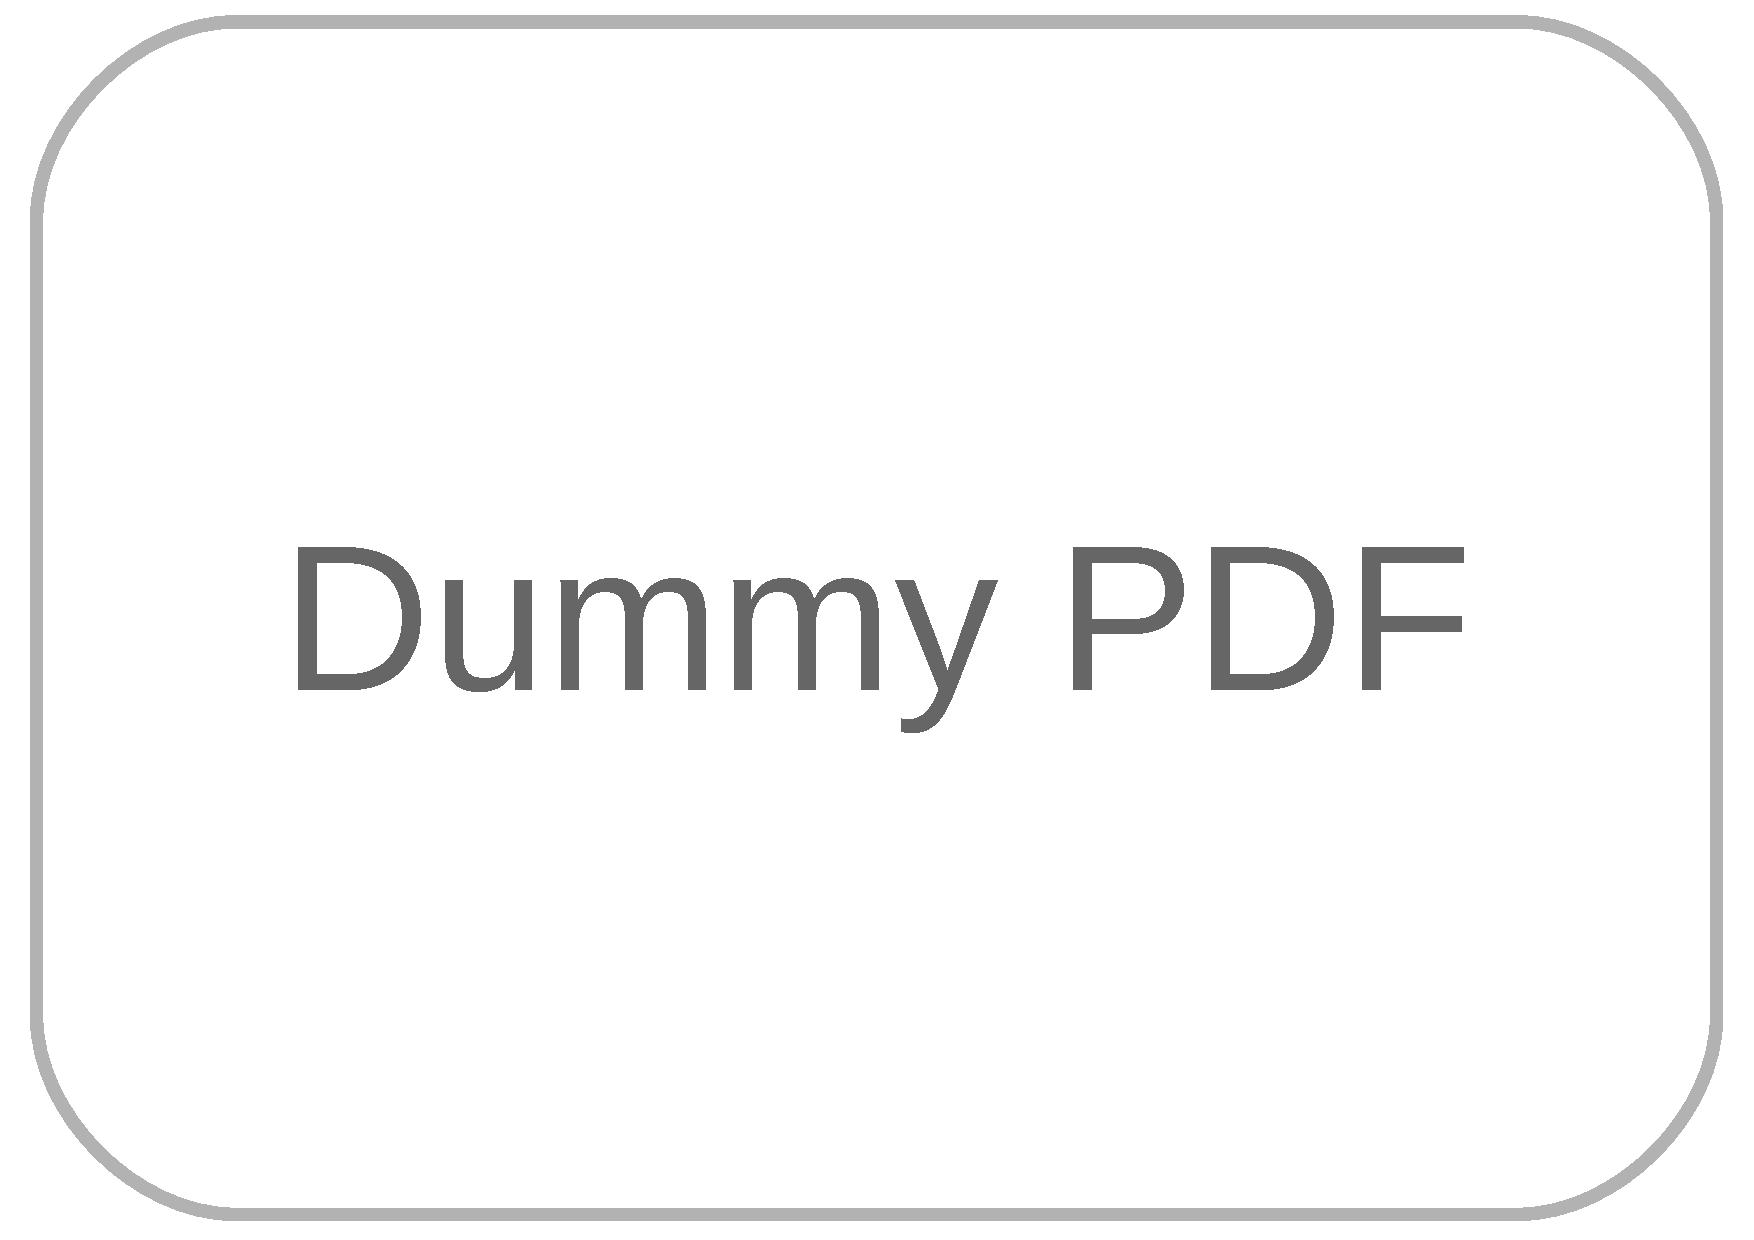
\includegraphics[width=0.5\textwidth]{pics/dummy.pdf}
\caption{Dummy PDF}
\label{fig:dummy}
\end{figure}
\newpage

\section{LowMC}
\section{Picnic}

\bibliographystyle{unsrt}
\bibliography{}



\end{document}
